\chapter{TLP modeling}
\section{Validation curves}
\label{apx:tlp-validation-curves}

\begin{figure}[!h]
  \centering
  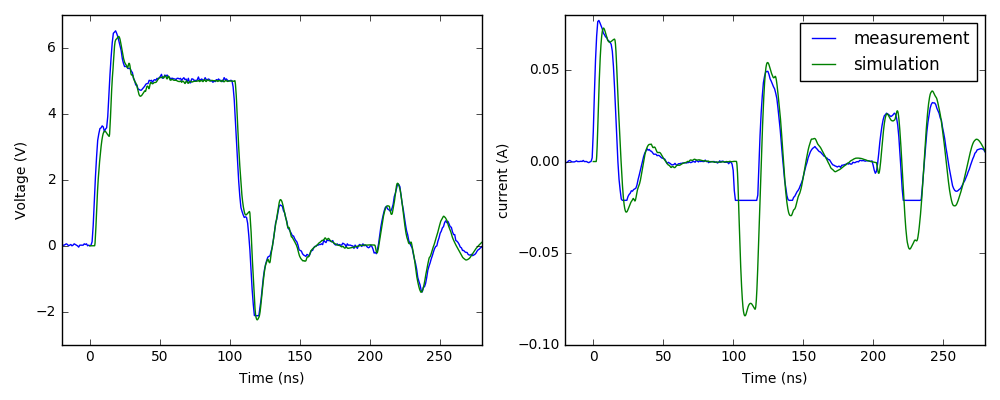
\includegraphics[width=\textwidth]{src/2/figures/tlp_comparison_open_10V.png}
  \caption{Voltage and current waveforms comparison : 10 V charging voltage on open circuit}
  \label{fig:comparison-tlp-open-10v}
\end{figure}

\begin{figure}[!h]
  \centering
  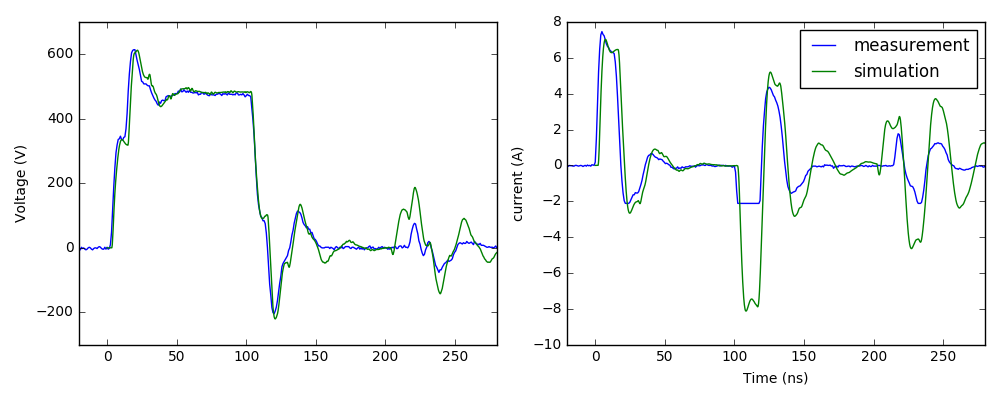
\includegraphics[width=\textwidth]{src/2/figures/tlp_comparison_open_1000V.png}
  \caption{Voltage and current waveforms comparison : 1000 V charging voltage on open circuit}
  \label{fig:comparison-tlp-open-1000V}
\end{figure}

\begin{figure}[!h]
  \centering
  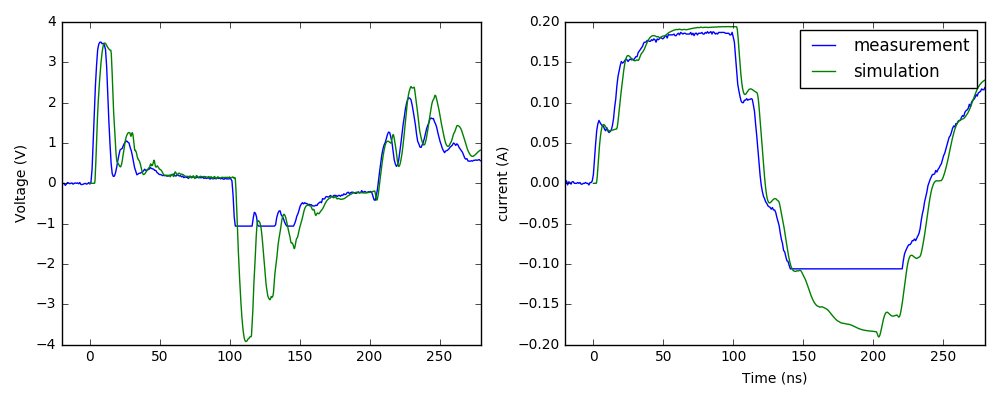
\includegraphics[width=\textwidth]{src/2/figures/tlp_comparison_short_10V.png}
  \caption{Voltage and current waveforms comparison : 10 V charging voltage on a short circuit}
  \label{fig:comparison-tlp-short-10V}
\end{figure}

\begin{figure}[!h]
  \centering
  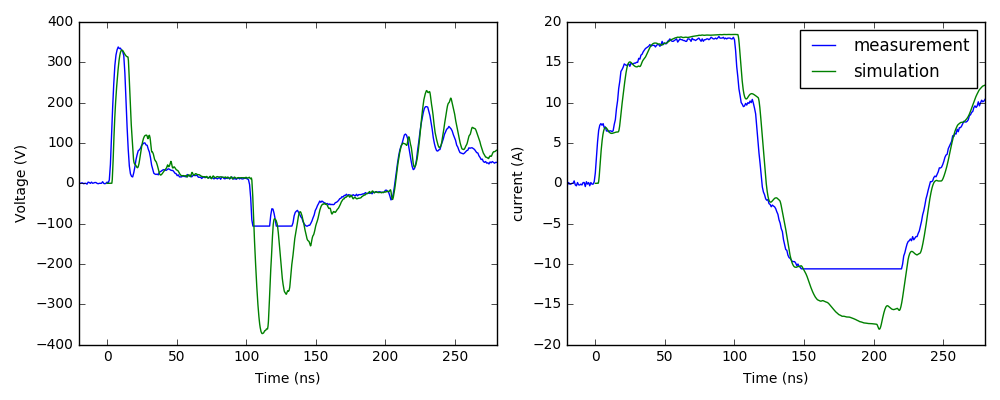
\includegraphics[width=\textwidth]{src/2/figures/tlp_comparison_short_1000V.png}
  \caption{Voltage and current waveforms comparison : 1000 V charging voltage on a short circuit}
  \label{fig:comparison-tlp-short-1000V}
\end{figure}

\begin{figure}[!h]
  \centering
  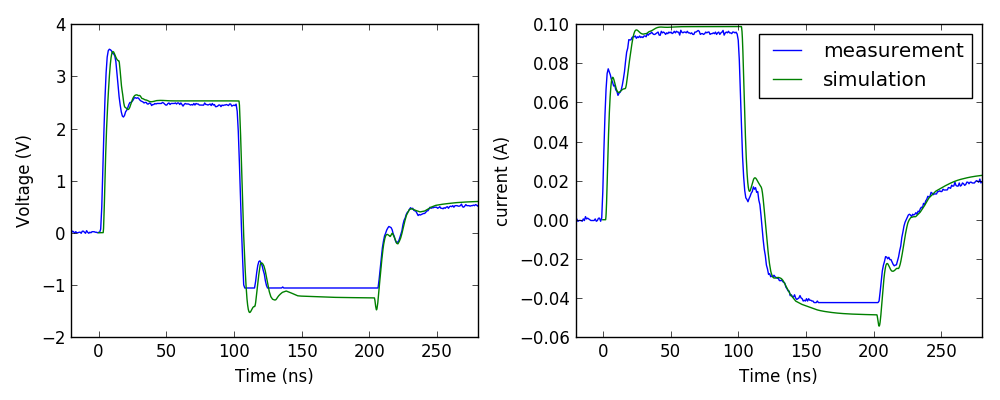
\includegraphics[width=\textwidth]{src/2/figures/tlp_comparison_R25_10V.png}
  \caption{Voltage and current waveforms comparison : 10 V charging voltage on 25\textOmega{}}
  \label{fig:comparison-tlp-load-10v}
\end{figure}

\begin{figure}[!h]
  \centering
  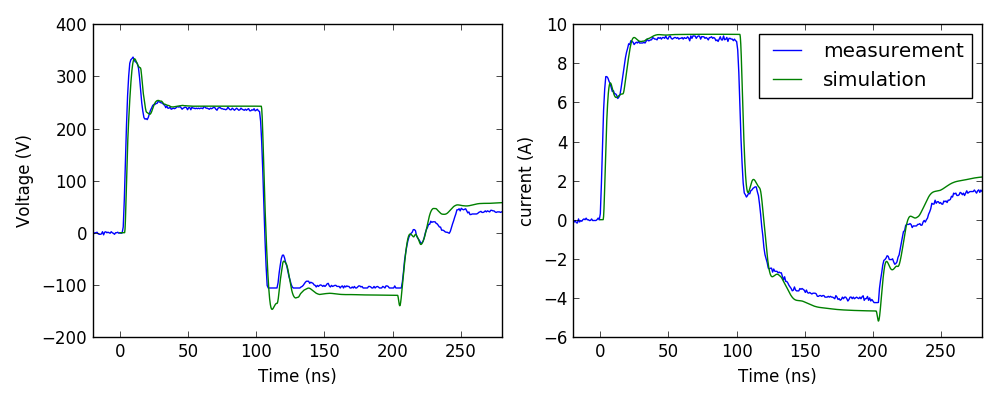
\includegraphics[width=\textwidth]{src/2/figures/tlp_comparison_R25_1000V.png}
  \caption{Voltage and current waveforms comparison : 1000 V charging voltage on 25\textOmega{}}
  \label{fig:comparison-tlp-load-1000v}
\end{figure}

\begin{figure}[!h]
  \centering
  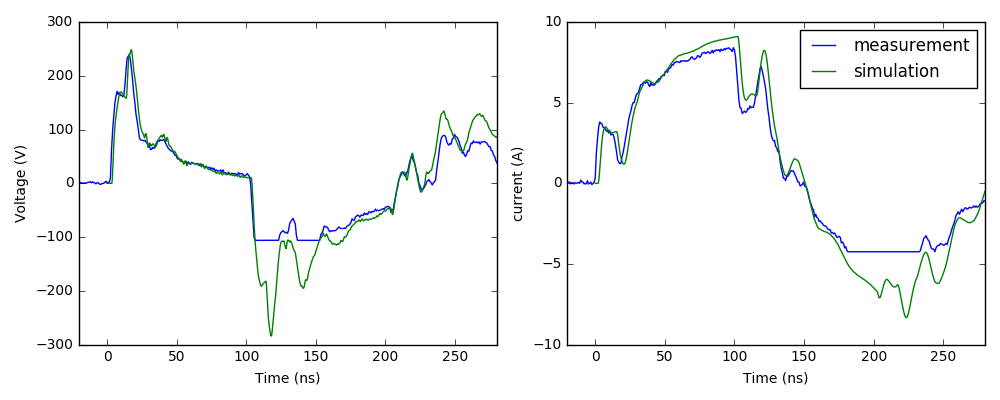
\includegraphics[width=\textwidth]{src/2/figures/tlp_comparison_470nH_500V.png}
  \caption{Voltage and current waveforms comparison : 500 V charging voltage on a 470nH inductor}
  \label{fig:comparison-tlp-inductor}
\end{figure}
